\documentclass[a4paper,12pt]{article} % тип документа

% report, book

% Рисунки
\usepackage{graphicx}
\usepackage{wrapfig}
\usepackage{mathtext}
\usepackage[left=2cm,right=2cm,
    top=2cm,bottom=2cm,bindingoffset=0cm]{geometry}

\usepackage{hyperref}
\usepackage[rgb]{xcolor}
\hypersetup{				% Гиперссылки
    colorlinks=true,       	% false: ссылки в рамках
	urlcolor=blue          % на URL
}

%  Русский язык
\usepackage[T2A]{fontenc}			% кодировка
\usepackage[utf8]{inputenc}			% кодировка исходного текста
\usepackage[english,russian]{babel}	% локализация и переносы
\addto\captionsrussian{\def\refname{Список используемой литературы}}


% Математика
\usepackage{amsmath,amsfonts,amssymb,amsthm,mathtools} 
\usepackage{titlesec}
\titlelabel{\thetitle.\quad}

\usepackage{wasysym}

\begin{document}\begin{titlepage}

\thispagestyle{empty}

\centerline{МОСКОВСКИЙ ФИЗИКО-ТЕХНИЧЕСКИЙ ИНСТИТУТ}
\centerline{(НАЦИОНАЛЬНЫЙ ИССЛЕДОВАТЕЛЬСКИЙ УНИВЕРСИТЕТ)}

\vfill

\centerline{\huge{Лабораторная работа 3.2.5}}
\centerline{\LARGE{<<Вынужденные колебания в электрическом контуре>>}}

\vfill

Студент группы Б02-109 \hfill Назарчук Анна

\vfill

\centerline{Долгопрудный, 2022}
\clearpage
\end{titlepage} 

\section{Аннотация}
В работе исследованы вынужденные колебания в электрическом контуре, рассчитана добротность контура различными способами. Измерения проведены на параллельном колебательном контуре с вынуждающей силой, меняющейся гармонически непрерывно или в форме цугов. Вычислены теоретическое значение добротности, добротность при измерении ширины резонансной кривой, значение при исследовании нарастания колебаний. Рассчитанные значения не совсем идентичны, предложены способы улучшения результатов.

\section{Введение}
Совсем несложно представить обычные детские качели. В зависимости от их строения, какие-то было легко раскачать, для каких-то требовались усилия. Но если начать двигаться с определенной частотой, то качели быстро начинают колебаться с большой амплитудой. Но, к сожалению, если перестать двигаться, то через некоторое время колебания станут совсем небольшими. Похожие явления наблюдаются и в электрических цепях, состоящих из катушек, резисторов, конденсаторов. Интересно, можно ли численно описать эти эффекты с помощью одной какой-то величины? Ответу на этот вопрос и наблюдению вышеописанных явлений в электрической цепи посвящена работа.

\section{Методика измерений}
\subsection*{Вводная часть}
<<Раскачкой>> электрической цепи называют вынужденные колебания, в работе рассмотрена вынуждающая сила, гармонически меняющаяся во времени. При подключении к контуру внешнего синусоидального источника в
нём возникают колебания, которые можно представить как суперпозицию
двух синусоид \cite{labnik} первая — с частотой собственных колебаний
контура и амплитудой, экспоненциально убывающей со временем; вторая
— с частотой внешнего источника и постоянной амплитудой. Со временем
собственные колебания затухают, и в контуре устанавливаются
вынужденные колебания. Зависимость амплитуды установившихся
колебаний от частоты внешнего сигнала называется резонансной
кривой. Ширина некоторой высоте (0.707 от максимальной) $\delta \omega$ определяет насколько близко необходимо подобраться к резонансной частоте $\omega_0$, чтобы достаточно сильно раскачать колебания в контуре, и называется добротностью:
\begin{equation}
\label{кривые}
Q=\frac{\omega_0}{\delta \omega}
\end{equation}

После этого необходимо рассмотреть установление колебаний, чтобы понять, как связана добротность контура с этим процессом:
\begin{figure}[h!]
\begin{center}
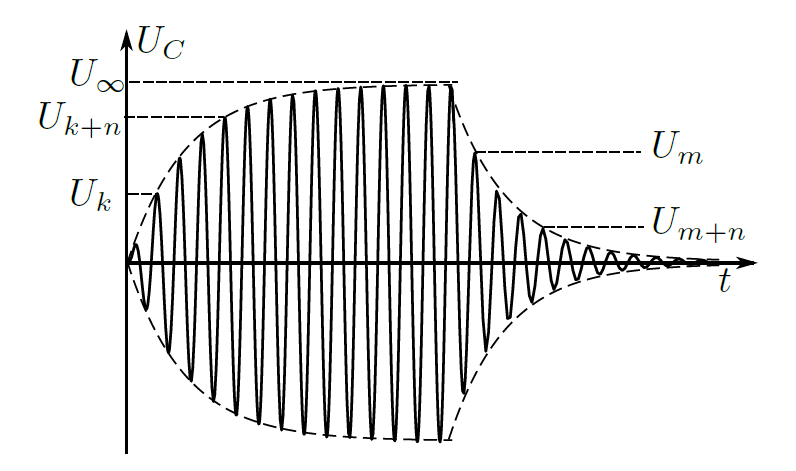
\includegraphics[width=0.55\textwidth]{затухание}
\caption{Нарастание и затухание вынужденных колебаний при подаче цугов (синусоидальные сигналы, разделенные временем без сигнала)} \label{затухание}.
\end{center}
\end{figure} 
Нарастание и затухание колебаний (рис. \ref{затухание}) можно наблюдать на
экране осциллографа, если на контур подаются цуги — отрезки синусоиды,
разделённые интервалами, в течение которых сигнал отсутствует. Теоретически известно, что \cite{labnik}, чем выше добротность, тем медленнее нарастают и медленнее затухают колебания в контуре. Получить значение Q можно по формуле \cite{labnik} (обозначения с рисунка \ref{затухание}):
\begin{equation}
\label{затух}
Q = \frac{\pi}{\frac{1}{n}ln(\frac{U_\infty-U_k}{U_\infty-U_{k+n}})}
\end{equation}
Более того, существует теоретическая формула для добротности (рассмотрен параллельный колебательный контур), которая следует из энергетического смысла добротности: 
В энергетическом смысле добротность $Q$ колебательной системы (механической, электрической, оптической и т. д.) определяется как отношение запасённой в ней энергии $W_0$ к потере $\Delta W$ энергии за время изменения фазы колебания
на 1 радиан.
\begin{equation}
Q = \frac{1}{R}\sqrt{\frac{L}{C}} 
\label{теор}
\end{equation}
\subsection*{Основная часть}
Получено три способа определения добротности (той самой характеристики, которая численно описывает явления затухания, резонанса колебаний), необходимо практически установить, приводят ли эти способы к одинаковому результату. Соответственно, работа состояла из нескольких частей: теоретический расчет добротности по формуле \ref{теор}, исследование резонансных кривых и процесса нарастания и затухания колебаний.

Исследование резонансных кривых проведено при генерации непрерывной синусоиды, при изменении частоты вынуждающих колебаний в разные стороны от резонансного значения. Построена зависимость амплитуды установившихся колебаний от частоты, из нее по формуле \ref{кривые} получена добротность.

Затухание и нарастание колебаний наблюдалось при генерации цугов - последовательности синусоидальных сигналов. В условиях резонанса, в которых и исследовалась система, затухание колебаний симметрично их нарастанию.


\subsection*{Экспериментальная установка}

Для генерации сигналов и вычисления добротности разными методами собрана экспериментальная установка (рис.  \ref{установка}. )
\begin{figure}[h!]
\begin{center}
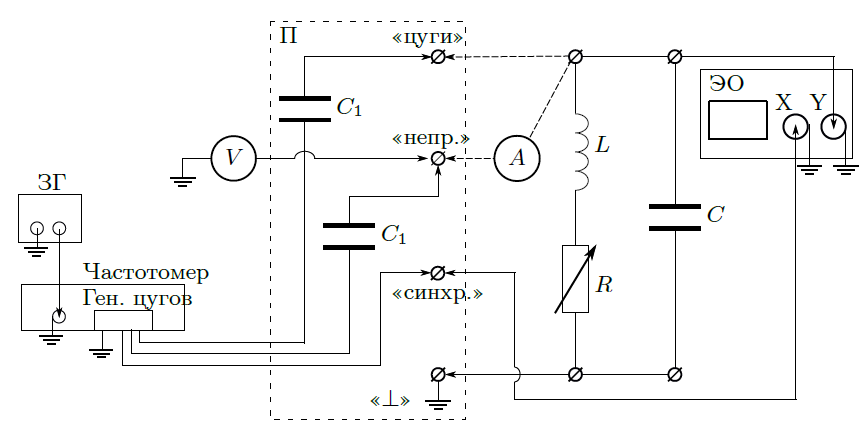
\includegraphics[width=0.95\textwidth]{установка}
\caption{Схема экспериментальная установка для исследования вынужденных
колебаний: ЗГ - звуковой генератор Г3-112, ген. цугов - генератор цугов ЧЗ-57, V - вольтметр В3-38, $R$ - магазин сопротивлений МСР-60, $L$ - магазин индуктивностей P567, ЭО - осциллограф GOS-620, П - панель} \label{установка}.
\end{center}
\end{figure} 

Колебательный контур состоял из конденсатора $С $ = 0.1 мкФ, катушки с индуктивностью $L$ = 100 мГн и магазина сопротивлений. Для измерения добротности необходимо было формировать как непрерывные синусоидальные сигналы (с помощью звукового генератора), так и цуги (с помощью генератора цугов). 

Для визуального наблюдения за процессом колебаний напряжение с конденсатора подано на вход электронного осциллографа. Чтобы картина на экране была устойчивой, частота развёртки осциллографа принудительно синхронизировалась с частотой повторения цугов. Для этого на генератор развёртки осциллографа подавались следующие с частотой повторения цугов управляющие импульсы, формируемые в блоке электронного реле, клемма «синхр.» которого смонтирована на панели. Эффективное значение напряжение на емкости C измерено с помощью вольтметра.

\section{Результаты и их обсуждение}
При непрерывной генерации синусоид получена резонансная кривая в относительных единицах (рис. \ref{график}). 

\begin{figure}[h!]
\begin{center}
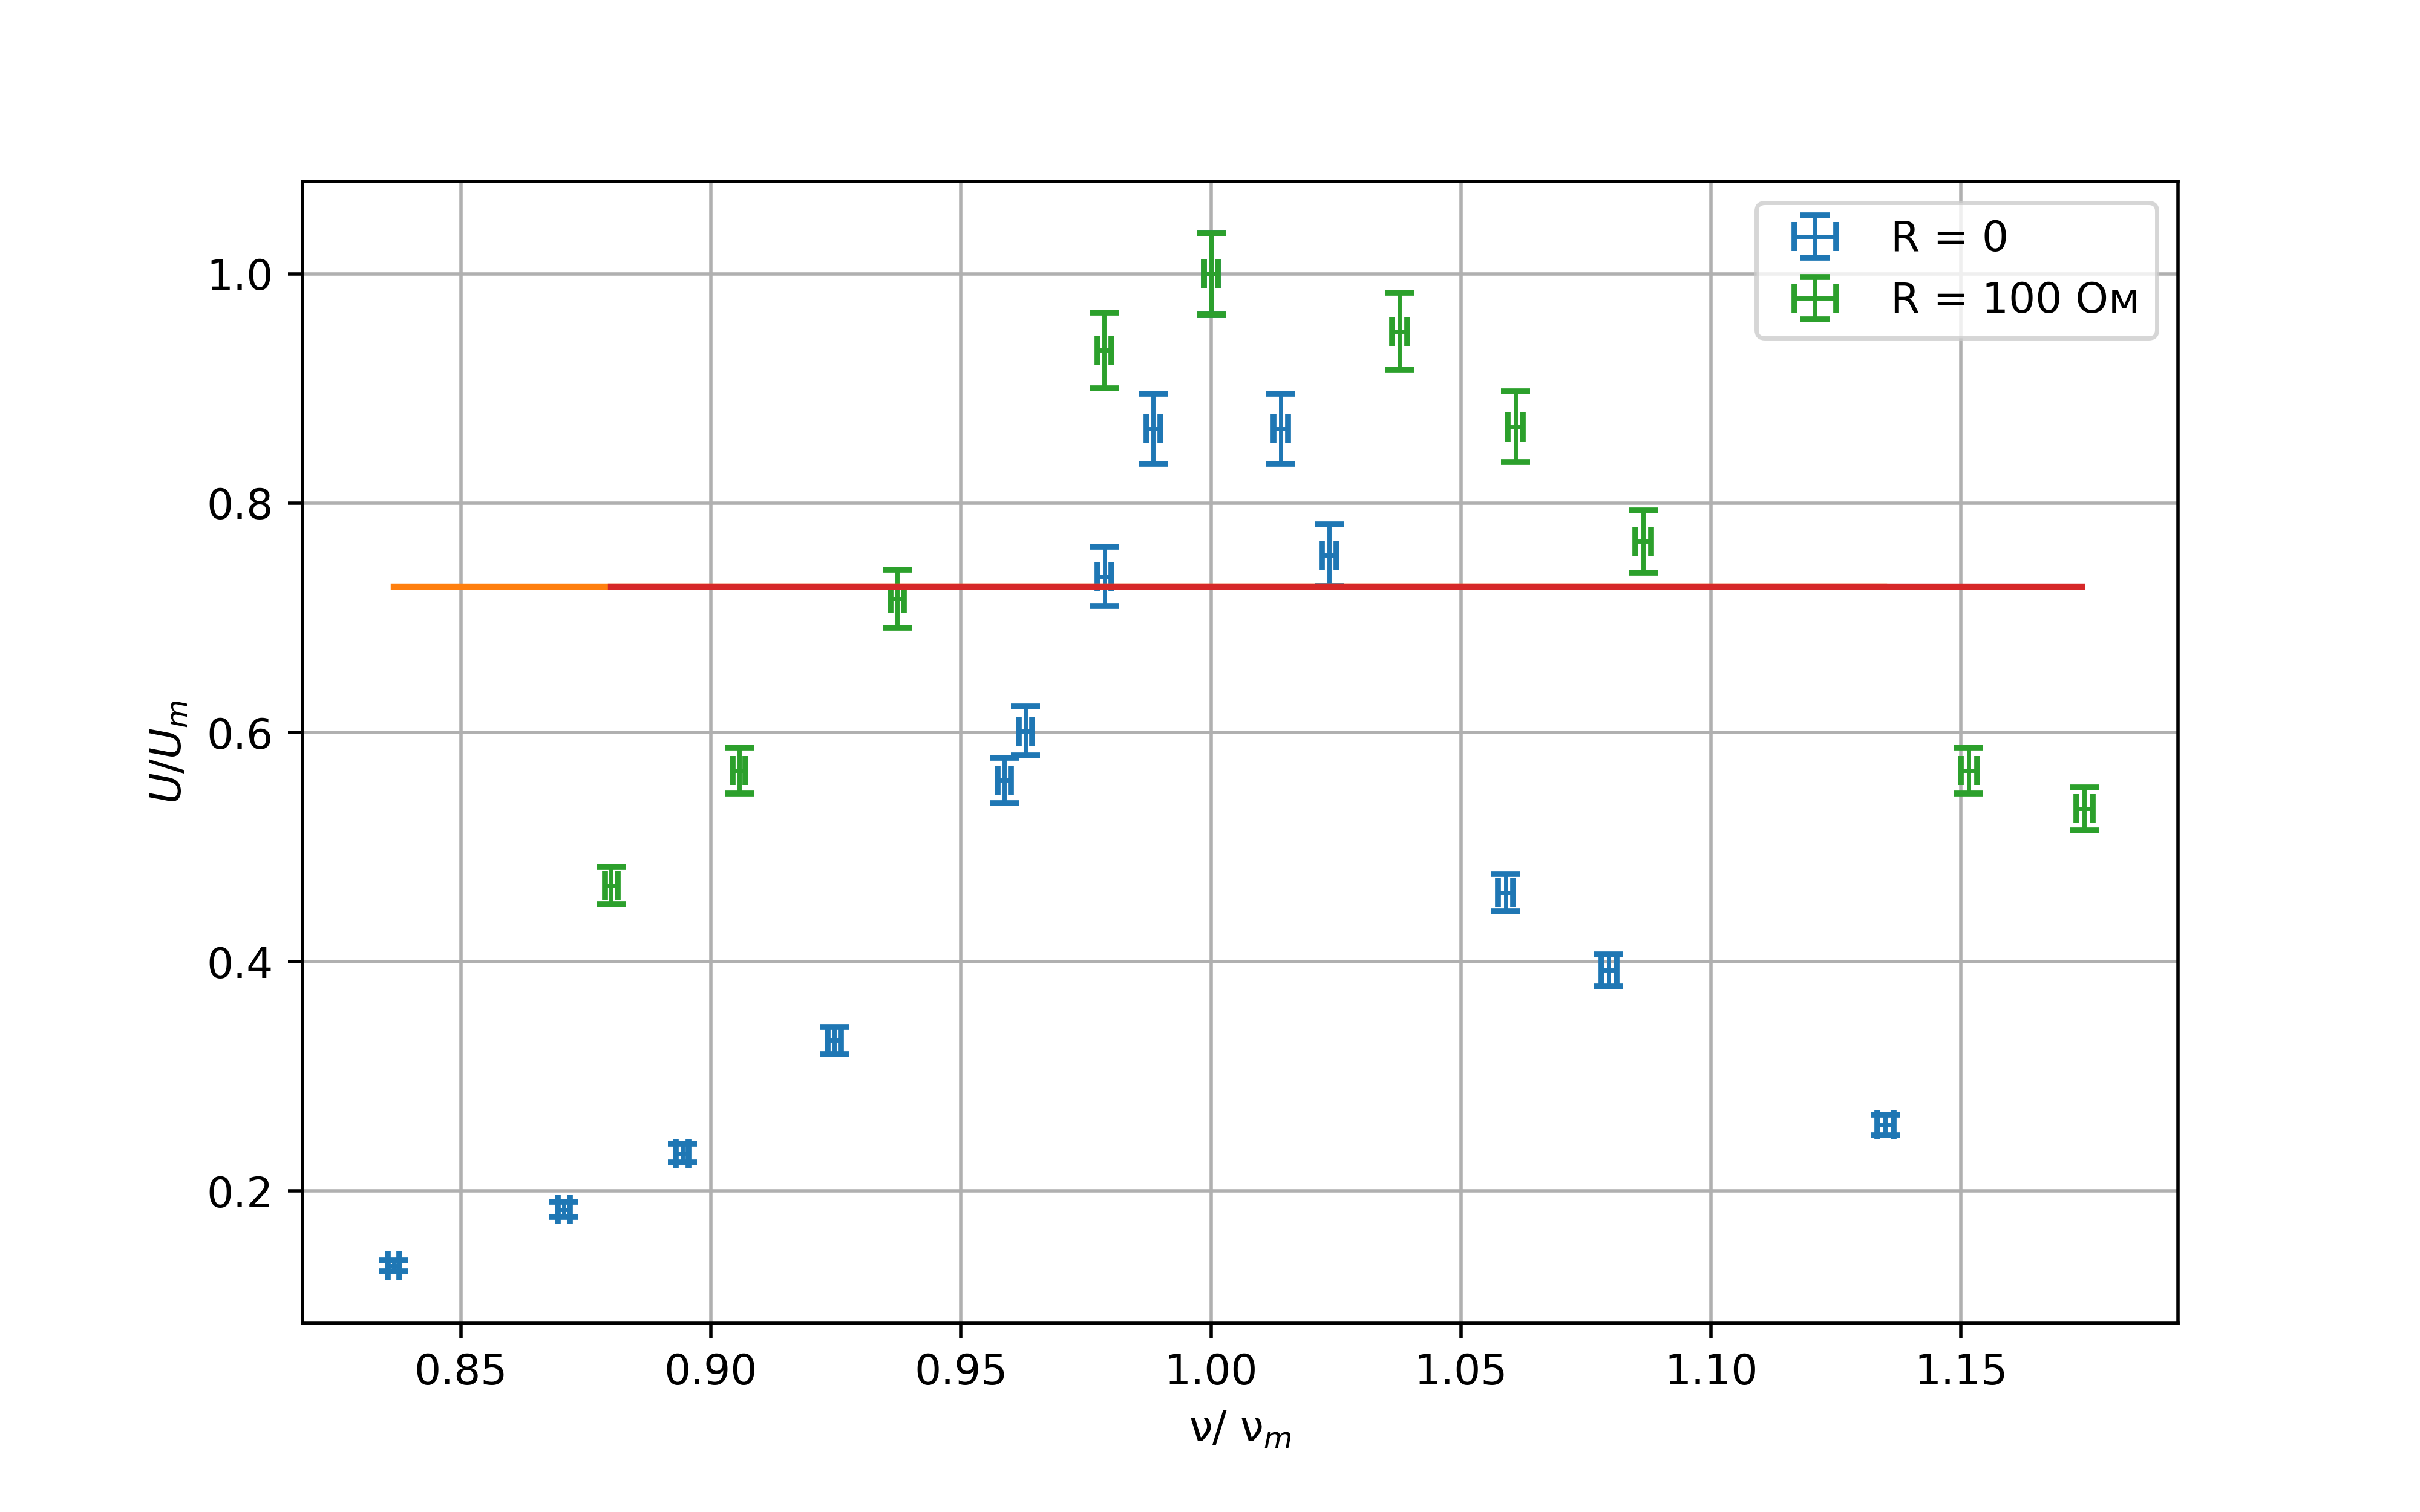
\includegraphics[width=0.95\textwidth]{graf}
\caption{Резонансная кривая в относительных единицах: $U/U_m$ - отношение амплитуды к резонансному значению, $\nu/\nu_m$ - отношение частоты к резонансному значению, для параллельного контура $С $ = 0.1 мкФ, $L$ = 100 мГн} \label{график}.
\end{center}
\end{figure} 

Вид зависимости схож с табличными представлениями резонансной кривой для параллельного контура \cite{labnik}. На высоте $U/U_m = 0.707$ вычислена ширина графика, рассчитана добротность системы (по формуле \ref{кривые}). (табл. \ref{кривые_табл}).
\begin{table}[h!]
\caption{Значение добротности системы при различных сопротивлениях, измерения методом резонансных кривых}
\label{кривые_табл}
\begin{tabular}{|l|l|l|}
\hline
R, Ом & Q     & $\sigma_Q$ \\ \hline
0     & 20.3 & 0.9       \\ \hline
100   & 6.3  & 0.4       \\ \hline
\end{tabular}
\end{table}

При генерации цуг на экране осциллографа получены картинки, похожие на рис. \ref{затухание}, однако они не абсолютно неподвижны для камеры, что не позволило запечатлеть их. Но измерены значения некоторых амплитуд колебаний при нарастании колебаний (результаты в приложении в табл.  \ref{нарост}). Так как в резонансе (при котором и проведено измерение) затухание и нарастание симметричны, нет необходимости вычислять амплитуды из обоих участков графика.

Из полученных данных по формуле \ref{затух} рассчитаны значения добротности (табл. \ref{затух_тбл}).
\begin{table}[h!]
\caption{Значение добротности системы при различных сопротивлениях, измерения методом исследования нарастания колебаний}
\label{затух_тбл}
\begin{tabular}{|l|l|l|}
\hline
R, Om & Q     & $\sigma_Q$ \\ \hline
0     & 22.5 & 2.1       \\ \hline
100   & 10.1 & 1.5       \\ \hline
\end{tabular}
\end{table}

По формуле \ref{теор} рассчитано теоретическое значение добротности контура:
\begin{table}[h!]
\caption{Значение добротности системы при различных сопротивлениях, теоретический расчет}
\label{теор_тбл}
\begin{tabular}{|l|l|l|}
\hline
R, Om & Q     & $\sigma_Q$ \\ \hline
0     & 33.5 & 1.0       \\ \hline
100   & 7.7 & 0.5       \\ \hline
\end{tabular}
\end{table}

Сведены рассчитанные значения добротности в единую таблицу \ref{един}.
\begin{table}[h!]
\caption{Результаты измерения добротности различными методами}
\label{един}
\begin{tabular}{|l|l|l|l|}
\hline
R, Om & $Q_{рез.крив.}$  & $Q_{затух.}$     & $Q_{теор.}$      \\ \hline
0     & 20.3 $\pm$ 0.9 & 22.5 $\pm$ 2.1 & 33.5 $\pm$ 1.0\\ \hline
100   & 6.3 $\pm$ 0.4  & 10.1 $\pm$ 1.5 & 7.7 $\pm$ 0.5    \\ \hline
\end{tabular}
\end{table}

Из таблицы видно, что данные не совсем совпадают, это можно объяснить методическими проблемами: резонансное значение частоты определяется не совсем точно (ручным способом), поэтому точки на резонансных кривых теряют в точности; еще число точек невелико, поэтому трудно определить ширину резонансной кривой на той или иной высоте. Также при нарастании колебаний амплитуды определяются из изображения на осциллографе, что также добавляет проблемности результату.

\section{Выводы}

\hspace{5mm}1. Из эксперементально полученных резонансных кривых, которые видом похожи на теоретически предсказанные, найдены добротность системы, из которых заметна высокодобротность контура ($Q\gg 1$).

2. Из исследования нарастания колебаний при резонансной частоте рассчитана добротность системы с большей погрешностью, нежели первым методом.

3. Сравнение экспериментальных значений добротности и теоретического ее расчета показал, что результаты не совсем близки друг к другу. Это объясняется проблемами в методике работы: большая часть измерений проведена вручную, из-за чего их небольшое количество и они имеют, возможно, не до конца верные значения. Данная проблема решается при внедрении автоматизации регистрации данных.



\begin{thebibliography}{}
    \bibitem{labnik}  Никулин М.Г., Попов П.В., Нозик А.А. и др. Лабораторный практикум по общей физике : учеб. пособие. В трех томах. Т. 2. Электричество и магнетизм
\end{thebibliography}


\section*{Приложение}
\begin{table}[h!]
\caption{Амплитуды некоторых колебаний при нарастании колебаний при генерации цугов}
\label{нарост}
\begin{tabular}{|l|l|l|l|l|}
\hline
$U_k$, mV & $U_{k+n}$, mV & $U_\infty$, mV & n & R=0 Om   \\ \hline
6         & 28            & 56             & 4 &          \\ \hline
5         & 21            & 43             & 4 &          \\ \hline
4         & 18            & 37             & 4 &          \\ \hline
3         & 12            & 26             & 4 &          \\ \hline
2         & 10            & 19             & 4 &          \\ \hline
$U_k$, mV & $U_{k+n}$, mV & $U_\infty$, mV & n & R=100 Om \\ \hline
2         & 5             & 7              & 3 &          \\ \hline
3         & 7             & 10.5           & 3 &          \\ \hline
4         & 10            & 13             & 3 &          \\ \hline
5         & 13            & 17.5           & 3 &          \\ \hline
7         & 18            & 25             & 3 &          \\ \hline
\end{tabular}
\end{table}

\end{document}
